\chapter{Radar solutions}
%Caratteristiche principali delle misurazioni radar for drone detection, %benefici e contro.
%Esempi di implementazioni radar possibili, stato dell'arte %(caratteristiche robin, informazioni pi\'u complete) 


%1. Radar position in surveillance systems. Pros and cons of radar for drone detection.
%2. Requirements for drone detection, example of FMCW solution 
%3. State of the art for drone detection (analysis of current radar solution).
%4. Definizione architettura e dimensionamento radar for drone detection to achieve the desirable goal.

In this chapter the radar drone detection technology is analyzed. For a better understanding, a general introduction to radar technologies is made and then follows a brief description of an example of radar technology (FMCW radar) choice considering the radar requirements for drone detection. Then the state of the art of solutions currently on the market are analyzed. 
In the end by using a 'top-down' approach a possible architecture of radar for drone detection is defined and dimensioned. 

\section{Radar technology}
Radar is one of the most widely used surveillance technology as it allows to measure the shape, the distance, the speed and the direction of arrival of the received reflected signal. To better understand where the radar is among the surveillance systems, we can divide surveillance technologies into two large groups: 
\begin{itemize}
     \item \textbf{Cooperative surveillance}: contain all techniques that rely on target devices, are included all technologies that need the cooperation of target to detect it. Is also subdivided in two other groups, dependent and independent type. The dependent cooperative surveillance systems do not perform any type of measurement and can only read information received from targets. The independent cooperative surveillance systems need only that target can reply to the messages, and for example by measuring the ToA the ground sensors can calculate it's horizontal position. 
         
    \item \textbf{Non cooperative surveillance}: include all techniques of surveillance that do not rely on target reply or target cooperation during the process of localization.
        
\end{itemize}

Considering the principle of operation of a radar, is simple to understand that it belongs to the typology of independent surveillance technologies. Then considering the mobility of a radar it's possible to classify them in rotatory radar or fixed radar. The first solution is characterized by a continuous rotation in azimuth performed by mechanical movements. While with the fixed radar an array of antennas is used to electronically scan the area, so the beam steering is performed only by changing the phases of elements.
It is useful to classify radars according to the number of quantities they are able to measure, considering the electronic or mechanical rotation also.
We can distinguish respectively 2D,3D and 4D radars.
\begin{itemize}
     \item \textbf{2D}: These are typically the less expensive configurations that can be implemented without the use of a phased array antenna. Mainly, there is only a mechanical rotation that allows you to scan the surrounding area in azimuth. In this case two dimensions can be measured: the slant range and the azimuth direction of arrival. An additional radar is delegated to obtain the information about the elevation of target, if needed.
         
    \item \textbf{3D}: With the use of phased array antennas technology, it is possible to combine mechanical azimuth scanning with vertical electronic scanning. This gives three dimensions that can be measured: the slant range, the azimuth arrival direction, and the elevation information.
    
    \item \textbf{4D}: In addition to the 3D measurements of distance, direction and vertical information this type of radar measures also the Doppler information. But also the 2D radar is capable to measure the Doppler information, so in general 4D is also a market name strategy. For simplicity we refer to a 4D radar as imaging radar or holographic radar that is able to reconstruct an image of observed situation. Usually these are used for automotive, in particular for driving assistance. The technology used is also the antenna phased array, both an horizontal and vertical array configuration. In this case the processing of received data is interested in electromagnetic pattern of received signal. A machine learning technique can be used to recognize the pattern of signals. The maximum range achievable with this technology is not too long, we are talking about several hundreds of meters.

\end{itemize}

Focusing on phased array antenna technology, two main implementations can be distinguished:

\begin{itemize}
     \item \textbf{PESA}: Passive Electronic Scanning Array is the configuration with a single transmitter/receiver linked to all the antenna elements by means of a phase shifter. In this way the only result achievable is the steering of the beam because only one single beam at one single frequency can be transmitted at time.

         
    \item \textbf{AESA}: Active Electronic Scanning Array is the configuration in which there are several transmitter/receiver, one for each element. In this way more complex action can be performed, for example more simultaneous beams at different frequency can be transmitted.
        
\end{itemize}



\begin{figure}
    \centering
    \subfloat[PESA]{{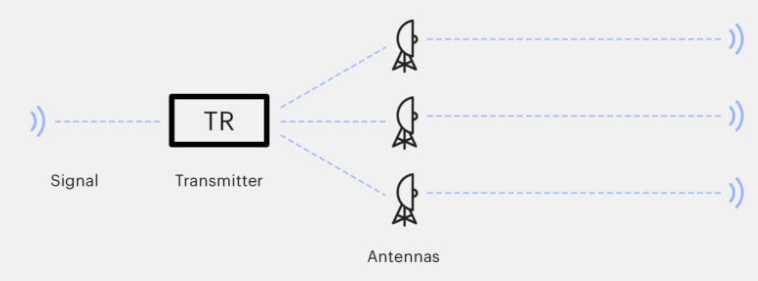
\includegraphics[width=10cm]{imgs/PESA radar.png} }}
    \qquad
    \subfloat[AESA]{{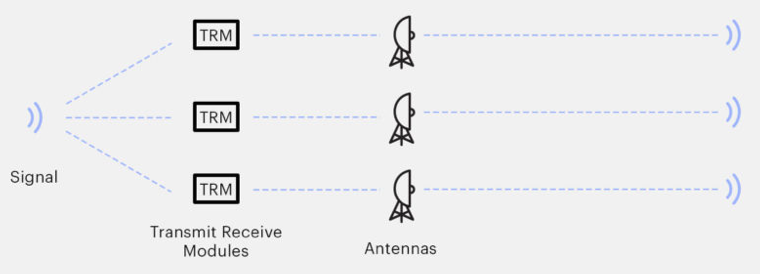
\includegraphics[width=10cm]{imgs/EASA radar.png} }}
    \caption{PESA vs AESA configurations.}
\end{figure}


In general, the configuration with vertically and horizontally arranged arrays (4D radars) used in conjunction with an FMCW technology is a promising solution for the drone detection case. \\ Another possible implementation of low cost radars is that of passive radars, PR. Exploiting the possible presence of the so-called Illuminators of Opportunity (IoP), in this way the presence of transmitters is completely eliminated, the architecture of the radar is greatly simplified and costs are also reduced. In this way the detection is completely based on the presence of radio signals transmitted by third party devices, such as digital television (DVB-T) and consequently it is not possible to design an appropriate waveform and cover contexts in which third party illuminators are not available.\\
Among the mentioned radar technologies, those that are of most interest for the application of drone detection are those with low cost, considering the treated context. Regarding the benefits and cons of the drone detection radar solution, early drone detection systems initially did not rely on radar technology due to the extremely low RCS of drones. Considering also that radar are primarily designed for bigger object like in the case of Primary Surveillance Radar. The main benefits of using a radar solution, as described in \cite{robinradar} are:
the large detection range in contrast with the range of the others solution precedent depicted. The constant tracking, that is a practice very advanced with radar which also enable the multiple targets tracking simultaneously. The possibility to track autonomous flying drones, which RF solution are not able to detect. The independence from weather conditions, which affect most of the previously seen solutions, such as IR/EO cameras. On the other hand the cons of this solution are: the detection range, in the end depends also on on the drone's dimensions, in fact it is directly proportional to RCS as is possible to understand by seeing the radar equation. The main difficulty is the distinction between a drone and any other flying object of the same size or a bird, in fact the classic radars are not able to distinguish them as in the case of PSR. The drone's small weight and their quickly acceleration make them possible to perform extreme maneuvering that make detection very difficult. Another cons is the band used and the related frequencies that are subject to regulation that varies from region to region. These must also be properly chosen to avoid interference as well. A brief summary of the pros and cons of the radar solution for drone detection is shown in the table \ref{tab:prosandcons}\\
\begin{table}[h!]
\centering
\begin{tabular}{|l|l|}
\hline
{\color[HTML]{000000} \textbf{Radar detection pro}}     & {\color[HTML]{000000} \textbf{Radar detection cons}}  \\ \hline
{\color[HTML]{000000} Long range detection}             & {\color[HTML]{000000} Low RCS drone}                \\ \hline
{\color[HTML]{000000} Drone autonomous flight}        & {\color[HTML]{000000} Distinction from birds}         \\ \hline
{\color[HTML]{000000} Constant tracking}                & {\color[HTML]{000000} Transmission frequency license} \\ \hline
{\color[HTML]{000000} Independence of visual condition} & {\color[HTML]{000000} Interference}                   \\ \hline
{\color[HTML]{000000} High accuracy localization}       & {\color[HTML]{000000} Low speed}                      \\ \hline
\end{tabular}
\caption{Pros and cons of drone's radar detection.}
\label{tab:prosandcons}
\end{table}

\newpage
%in seguito i benefici e i contro della soluzione radar for drone detection.
\section{Requirements and FMCW radar}
Having defined the operational environment and the features of drones in the previous chapter, a first analysis of the general requirements for a radar is made. The first two fundamental needs to reveal a drone concern the Radar Cross Section and the Doppler analysis. Since the dimensions of drones are very small, typical values of RCS are in the order of 0.01 - 0.03 square meters \cite{rcsdrone}. So, as mentioned in the previous chapter it's necessary that frequency belongs to bands that goes from 8 to 20 GHz. Concerning the velocity measurements, a continuous wave radar is able to measure the velocity using the Doppler information. Being interested in both distance and speed measurement a frequency modulated continuous wave radar (FMCW) is one of the possible solutions. Considering also that is necessary a further Doppler processing during the detection that help to distinguish moving target and solve the problem of primary identification. The measurement related to the detection must be processed by micro Doppler analysis and then compared to a model \cite{microdoppler_and_SVM}. This task requires additional time which is added to the standard time of detection, so unlike a PSR (Primary Surveillance Radar) in this case the detection time could be greater. So, one of the objective can be to reduce at the minimum the time of detection while keeping the level of accuracy acceptable.\\ Another important consideration is about the maximum power transmitted, considering the near presence of people, it must be not so high and it is another motivations to use a FMCW radar that is characterized by a low peak power. Thinking about the radar architecture, a monostatic configuration can be a useful solution considering the requirements of portability for public environment. In figure \ref{FMCWradarchain} a typical FMCW radar chain is shown. 

\begin{figure}[h!]
    \centering
    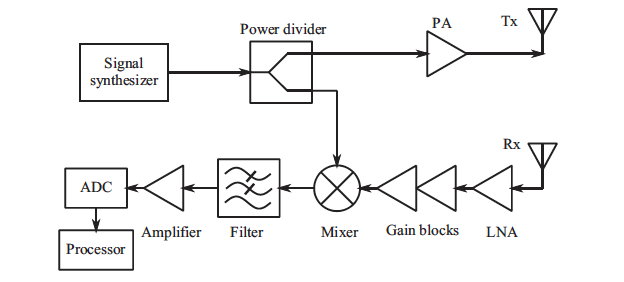
\includegraphics[width=13cm]{imgs/FMCW radar chain.png}
    \caption{FMCW radar chain.}
    \label{FMCWradarchain}
\end{figure}
In this configuration the isolation between transmission and reception antenna is not perfect so considering also the antenna mismatch  is possible to use a Reflected Power Canceller (RPC) in addition to the classical radar chain. 
It is possible to observe that the phase reference is maintained known and a coherent detector is used, then the reflected signals received is analyzed in the spectral domain and starting from frequency variations, velocity and distances are measured. To do this a Fast Fourier Transform is used. So the FMCW radar represents a possible candidate for the solution of the drone detection problem. It is therefore appropriate to better analyze its characteristics. The typical signal used by this type of radar is a chirp signal characterized by a linear change in frequency over time. In this way the reflected echo mixed with the transmitted signal will produce a frequency difference called beat frequency and knowing the time-relation of this frequency is possible to obtain the range and velocity quantities. It's possible to demonstrate that higher the bandwidth means higher the range resolution. On the other hand, by increasing the modulation period at equal bandwidth means a lower frequency to measure and an higher frequency resolution. An example of linear frequency modulation is shown below. 

\begin{figure}[h!]
    \centering
    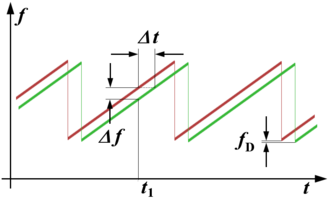
\includegraphics[width=8cm]{imgs/Fmcw modulation.png}
    \caption{FMCW modulation}
\end{figure}

The advantages of FMCW radar respect to a classic pulsed radar are:

\begin{itemize}

    \item \textbf{Low peak power}: there is no standby period and so the transmitted power is linearly spreaded among the channel, this means also a low probability of intercept; 
         
    \item \textbf{Higher bandwidth}: its possible to demonstrate that higher the bandwidth of modulation means higher the range resolution; 
    
    \item \textbf{Short-range detection}, no blind spot in front of the radar because there is continuous transmission and reception unlike a pulsed radar;

    \item \textbf{Low cost receiver}, because IF bandwidth related to sampling frequency is minor than total bandwidth of  chirp;
    
    \item \textbf{Radar dimensions}, typical implementations of this radar are very small and give the possibility to create a radar through off the shelf components ;
        
\end{itemize}

\section{State of the art for radar drone detection system}
Follow a brief description of current solutions that it's possible to find on the market, but most of these solutions are either of military level and/or expensive. 
\subsection{Robin Radar, Elvira and Iris}
Some solutions offered by Robin Radar make use of FMCW radar technology.  In particular, two solutions are offered, respectively called IRIS and ELVIRA, the first more expensive 3D type and the second less expensive 2D type. The radars in question are capable of doing tracking, multi target detection and micro Doppler analysis. In addition, the lightest solution in this case comes to weigh 25 kg and has dimensions of 55x62 cm. So it is also considerable as portable solution but it's possible to find lighter and smaller solutions for extreme portability needs. As can be seen from the specifications shown in the table \ref{tab:robinradar}, the technique used to distinguish a drone from another object or bird is that of micro Doppler analysis.

\begin{table}[h!]
\centering
\begin{tabular}{|
>{\columncolor[HTML]{FFFFFF}}l |
>{\columncolor[HTML]{FFFFFF}}l |
>{\columncolor[HTML]{FFFFFF}}l |}
\hline
{\color[HTML]{000000} \textbf{SPEC}}         & {\color[HTML]{000000} \textbf{IRIS}}          & {\color[HTML]{000000} \textbf{ELVIRA}}        \\ \hline
{\color[HTML]{000000} Technology}            & {\color[HTML]{000000} FMCW}                   & {\color[HTML]{000000} FMCW}                   \\ \hline
{\color[HTML]{000000} Frequency}             & {\color[HTML]{000000} X-Band (8900-9650 MHz)} & {\color[HTML]{000000} X-Band (8700-9650 MHz)} \\ \hline
{\color[HTML]{000000} Power Output}          & {\color[HTML]{000000} 2 x 12 Watt}            & {\color[HTML]{000000} 4 Watt}                 \\ \hline
{\color[HTML]{000000} Instrument Range}      & {\color[HTML]{000000} 5 km}                   & {\color[HTML]{000000} 5 km}                   \\ \hline
{\color[HTML]{000000} Detection Range}       & {\color[HTML]{000000} 4 km}                   & {\color[HTML]{000000} 2.7 km}                 \\ \hline
{\color[HTML]{000000} Classification Range}  & {\color[HTML]{000000} 2.2 km}                 & {\color[HTML]{000000} 1.8 km}                 \\ \hline
{\color[HTML]{000000} Main Beam Width}       & {\color[HTML]{000000} 6\degree x 60\degree}             & {\color[HTML]{000000} 10\degree x 10\degree}            \\ \hline
{\color[HTML]{000000} Rotation}              & {\color[HTML]{000000} 30 rpm}                 & {\color[HTML]{000000} 46 rpm}                 \\ \hline
{\color[HTML]{000000} Classification Method} & {\color[HTML]{000000} Micro-Doppler}          & {\color[HTML]{000000} Micro-Doppler}          \\ \hline
{\color[HTML]{000000} Range Accuracy}        & {\color[HTML]{000000} 0.6 m}                  & {\color[HTML]{000000} 0.6 m}                  \\ \hline
{\color[HTML]{000000} Azimuth Accuracy}      & {\color[HTML]{000000} 0.6\degree}                  & {\color[HTML]{000000} 1\degree}                    \\ \hline
\end{tabular}
\caption{Robin radar specification.}
\label{tab:robinradar}
\end{table}
\newpage
For what concern the 3D solution, the maximum range in which a drone the size of a DJI Inspire can be detected is 4 km. In contrast, the maximum range within which a drone can be classified and distinguished from a bird is only 2.2 km. In this case, the configuration used for the antenna is a linear array type. As it is possible to observe in figure \ref{irisimg} there are four rotating arrays (30 rpm). In fact, counting the number of elements that make up each array and considering the frequency used, it is possible to calculate the width of the beam in elevation. If we consider that each element is placed at $\lambda/2$  and each has a width of about 1 cm, the width of the beam is about 6\degree.

\begin{figure}[h!]
    \centering
    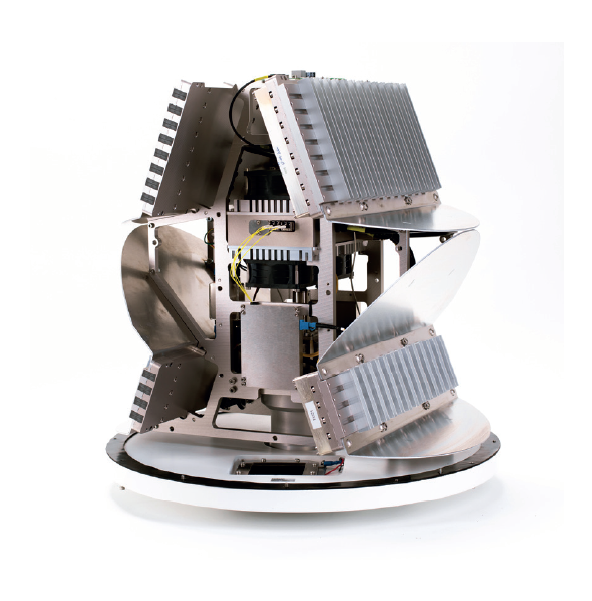
\includegraphics[width=8cm]{imgs/IRIS robin.png}
    \caption{IRIS arrays configuration.}
    \label{irisimg}
\end{figure}

For what concern the 2D radar a heavier solution has been considered, of about 75 kg. Consequently, this configuration makes this solution less suitable for extreme portability situation. On the other hand, in this case there is a much lower power consumption and the detection range is 1.3 km smaller than the 3D configuration. Also the width of the main beam in azimuth is smaller than in the previous case, it is equal to 10 degrees both in azimuth and in elevation. In fact is necessary a rotation velocity of 45 rpm to achieve a good result of accuracy in front of a reduced beamwidth. 

\subsection{Aveillant, Gamekeeper 16U}
Another interesting solution is that offered by Aveillant, which specializes in holographic radar design. The technology used here deviates greatly from the simple linear arrays just seen and is based on the technology previously mentioned as 4D radar. The goal is to reconstruct a 3D image of the surrounding environment based on the pattern waveform information collected at the radar. This solution is not addicted for portable needs, in fact the weight is about 370 kg and dimensions are 3.5 m x 0.95 m x 0.4 m. Considering also the high power consumption is not considered as a low cost solution. The specifications and performance are shown below.

\begin{table}[h!]
\centering
\begin{tabular}{|
>{\columncolor[HTML]{FFFFFF}}l |
>{\columncolor[HTML]{FFFFFF}}l |}
\hline
{\color[HTML]{000000} \textbf{SPEC}}      & {\color[HTML]{000000} \textbf{Gamekeeper 16U}}   \\ \hline
{\color[HTML]{000000} Technology}         & {\color[HTML]{000000} Holographic radar}         \\ \hline
{\color[HTML]{000000} Frequency}          & {\color[HTML]{000000} L-Band}                    \\ \hline
{\color[HTML]{000000} Power Output}       & {\color[HTML]{000000} 2 kW}                      \\ \hline
{\color[HTML]{000000} Instrument Range}   & {\color[HTML]{000000} 7.5 km}                    \\ \hline
{\color[HTML]{000000} Detection Range}    & {\color[HTML]{000000} 5 km}                      \\ \hline
{\color[HTML]{000000} Target RCS}         & {\color[HTML]{000000} 0.01 m\textasciicircum{}2} \\ \hline
{\color[HTML]{000000} Range in Altitude}  & {\color[HTML]{000000} 900 m}                     \\ \hline
{\color[HTML]{000000} Azimuth Coverage}   & {\color[HTML]{000000} 90\degree}                      \\ \hline
{\color[HTML]{000000} Elevation Coverage} & {\color[HTML]{000000} 30\degree}                      \\ \hline
{\color[HTML]{000000} Range Accuracy}     & {\color[HTML]{000000} 0.6 m}                     \\ \hline
{\color[HTML]{000000} Azimuth Accuracy}   & {\color[HTML]{000000} 0.6\degree}                     \\ \hline
\end{tabular}
\caption{Gamekepeer 16U specifications.}
\label{tab:gamekeeper}
\end{table}

\begin{figure}[h!]
    \centering
    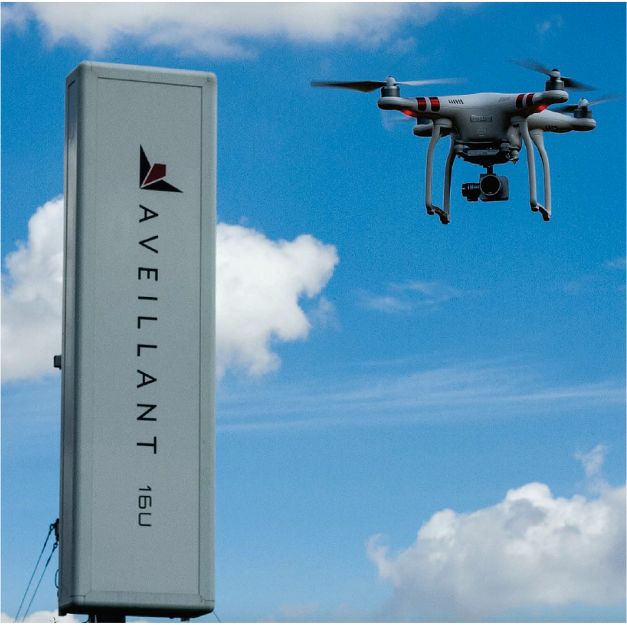
\includegraphics[width=6cm]{imgs/Gamekeeper 16U.png}
    \caption{Gamekeeper 16U.}
    \label{gamekeeperimg}
    
\end{figure}


To better understand how this radar work is necessary to explain the holographic principle on which it is based, discover by Gabor in 1948 \cite{holographic}. Both the spatial and temporal information of an electromagnetic wave are imprinted in the phase. In fact, it is possible to express it as: $\phi=\omega t+\boldsymbol{k} \boldsymbol{z}+\phi_{0}$
Unfortunately, it is not possible to save directly the visible light phase in any way, due to the higher frequency (hundreds of THz). Holograms are just used for this, thanks to an interference they can record the phase information. Using a reference wave, the interference that occurs between the echo reflected by the target and that of the reference wave is imprinted on a film. Then, the film is illuminated with the reference wave and thanks to the phenomenon of diffraction is produced a mirror wave to that reflected by the target. The same principle is reproduced with radars where the film surface is seen like a receiver array where each element can calculate the phase difference between a reference wave and a received wave. For example, is possible to use a power splitter to divide the 'reference wave', that remains in radar and is used to demodulate the received signal and the 'illuminated wave', that is amplified and radiated by the antenna. In this case the interference between the echo signal and the reference wave took place in the demodulator instead of a metallic film. This mode of operation is very similar to that used by an FMCW radar, where the transmitted and received signals are mixed together and the result is a signal at a beat frequency.

\subsection{Kelvin Hughes, Spexer360}
Regarding other radar technologies, is possible also to identify the one offered by Kelvin Hughes that is based on a solid-state pulse radar. The technology is based on Sharp Eye, a class of radars developed by the same company, the main feature of this radar is the compactness, thanks to the small size is easily deployable and can be carried by a man on foot. Usually is combined with electro optic cameras to achieve high performance against drones. To achieve a good result in detect small aerial vehicle is crucial the post processing, are implemented the pulse compression, the Doppler analysis and the adaptive clutter suppression techniques. The dimension of rotating antenna is of 522 mm. Follow a recap of specification available of this solution (table \ref{spexerspec}).

\begin{table}[h!]
\centering
\begin{tabular}{|
>{\columncolor[HTML]{FFFFFF}}l |
>{\columncolor[HTML]{FFFFFF}}l |}
\hline
{\color[HTML]{000000} \textbf{SPEC}}        & {\color[HTML]{000000} \textbf{Spexer 360}}        \\ \hline
{\color[HTML]{000000} Technology}           & {\color[HTML]{000000} Solid State Pulse Radar}    \\ \hline
{\color[HTML]{000000} Frequency}            & {\color[HTML]{000000} X-Band {[}9.22-9.38 GHz{]}} \\ \hline
{\color[HTML]{000000} Power Output}         & {\color[HTML]{000000} 80 W}                       \\ \hline
{\color[HTML]{000000} Instrument Range}     & {\color[HTML]{000000} 2.4 km}                     \\ \hline
{\color[HTML]{000000} Target RCS}           & {\color[HTML]{000000} 0.03 m\textasciicircum{}2}  \\ \hline
{\color[HTML]{000000} Range accuracy}       & {\color[HTML]{000000} 5 m  RMS}                   \\ \hline
{\color[HTML]{000000} Azimuth accuracy}     & {\color[HTML]{000000} 0.8\degree  RMS}                 \\ \hline
{\color[HTML]{000000} Azimuth Beam Width}   & {\color[HTML]{000000} \textless{}4.0\degree}            \\ \hline
{\color[HTML]{000000} Elevation Beam Width} & {\color[HTML]{000000} 25\degree}                       \\ \hline
{\color[HTML]{000000} Range Accuracy}       & {\color[HTML]{000000} 0.6 m}                      \\ \hline
{\color[HTML]{000000} Azimuth Accuracy}     & {\color[HTML]{000000} 0.6\degree}                      \\ \hline
\end{tabular}
\caption{Spexer360 specifications.}
\label{spexerspec}
\end{table}

In figure \ref{spexerimg} is shown a typical installation with electro optic cameras.

\begin{figure}[h!]
    \centering
    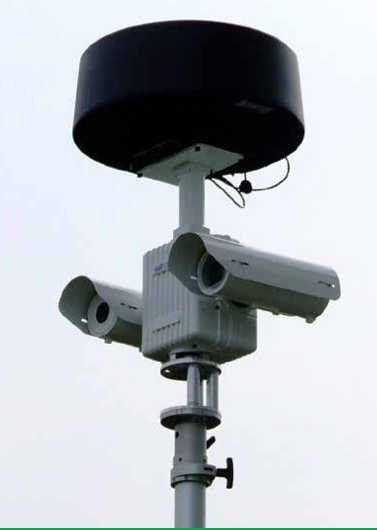
\includegraphics[width=4cm]{imgs/Kelvin hughes .png}
    \caption{Spexer 360 installation.}
    \label{spexerimg}
\end{figure}
\newpage
\subsection{Droneshield, RadarZero}
One of the solutions closest to the needs of our cause is that offered by the company Droneshield, called RadarZero. This company is specialized in drone detection and contrast solutions, they have also produced a wearable RF detector that is completely passive and weighs only 700 g, addicted to military environments it is able to detect a cooperating drone. The RadarZero is the most compact solution observed so far, as big as a notebook (20 cm x 16 xm x 5.6 cm). Moreover, it provides a relaxed range constraint of about maximum 1 km as detection range. It seems to be the most promising solution considering the ease of transport, use, installation and cost. In fact, it does not seem to be a solution designed for military cases, but it is perfectly suited to civilian and private contexts. It has been successfully demonstrated with the TIPS-C (Trakka Interceptor Package Solution) system at Eglin Air Force Base. In figure \ref{radarzero} is shown the typical installation of RadarZero, in this case is possible to observe four module each one covering 90 degrees, and other optical system. The interesting fact is that it requires no initial calibration and transmits very low power.

\begin{figure}[h!]
    \centering
    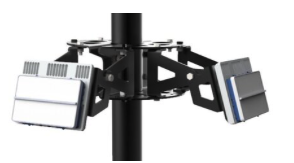
\includegraphics[width=8cm]{imgs/RadarZero installation.png}
    \caption{RadarZero installation.}
    \label{radarzero}
\end{figure}

\newpage


\begin{table}[]
\centering
\begin{tabular}{|
>{\columncolor[HTML]{FFFFFF}}l |
>{\columncolor[HTML]{FFFFFF}}l |}
\hline
{\color[HTML]{000000} \textbf{SPEC}}      & {\color[HTML]{000000} \textbf{Droneshield Radar Zero}} \\ \hline
{\color[HTML]{000000} Technology}         & {\color[HTML]{000000} -}                               \\ \hline
{\color[HTML]{000000} Frequency}          & {\color[HTML]{000000} K band (24.45 - 24.65 GHz)}      \\ \hline
{\color[HTML]{000000} Power Output}       & {\color[HTML]{000000} 3.4 W}                           \\ \hline
{\color[HTML]{000000} Instrument Range}   & {\color[HTML]{000000} 1 km}                            \\ \hline
{\color[HTML]{000000} Target RCS}         & {\color[HTML]{000000} -}                               \\ \hline
{\color[HTML]{000000} Range in Altitude}  & {\color[HTML]{000000} -}                               \\ \hline
{\color[HTML]{000000} Azimuth Coverage}   & {\color[HTML]{000000} 80\degree}                             \\ \hline
{\color[HTML]{000000} Elevation Coverage} & {\color[HTML]{000000} 90\degree}                             \\ \hline
{\color[HTML]{000000} Azimuth Accuracy}   & {\color[HTML]{000000} 1\degree}                             \\ \hline
\end{tabular}
\caption{RadarZero specifications.}
\label{radarzerospec}
\end{table}

In table \ref{radarzerospec} the specifications available is shown.
Unfortunately, the information about the radar technology used by RadarZero is not know and is possible only to derive and suppose it.

\subsection{Advance Protection System, FIELDCtrl Access}
Advance Protection System (APSsystem), work in the protection of airspace and offers different solutions in the field of drone defense specialized in ultra precise 3D MIMO radars. They designed several radar solutions by gradually increasing performance and cost. The entry level and less expensive solution is the FIELDCtrl Access, with a detection range of 2 km and AESA e MIMO (Multiple Input Multiple Output) technology for antennas. A typical antennas configuration and radar housing is shown in figure \ref{CTRLantenna}.

\begin{figure}[h!]
    \centering
    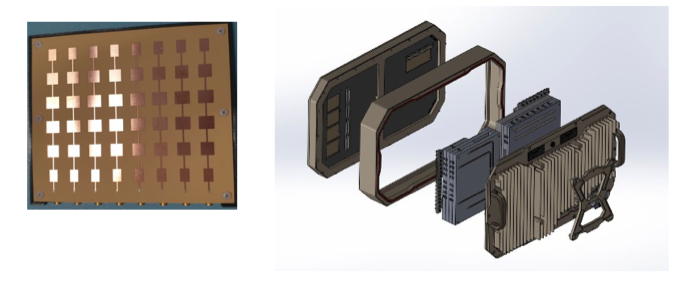
\includegraphics[width=13cm]{imgs/Ctrl acces antenna.png}
    \caption{FIELDCtrl Antennas.}
    \label{CTRLantenna}
\end{figure}

Below are shown the specification of this configuration (table \ref{FIELDctrltab}), the results are more interested for our cause because the design and implementation of a  2D array patch antenna like this is very powerful and cheap thanks to the technological improvements in this field. On the other side, management and processing of information coming from MIMO configuration like this is very challenging and is the more expensive part. 
\begin{table}[h!]
\centering
\begin{tabular}{|
>{\columncolor[HTML]{FFFFFF}}l |
>{\columncolor[HTML]{FFFFFF}}l |}
\hline
{\color[HTML]{000000} \textbf{SPEC}}             & {\color[HTML]{000000} \textbf{FIELDctrl Access}} \\ \hline
{\color[HTML]{000000} Technology}                & {\color[HTML]{000000} 3D MIMO/AESA}              \\ \hline
{\color[HTML]{000000} Frequency}                 & {\color[HTML]{000000} X-Band}                    \\ \hline
{\color[HTML]{000000} Power Output}              & {\color[HTML]{000000} 2 kW}                      \\ \hline
{\color[HTML]{000000} Instrument Range}          & {\color[HTML]{000000} 7 km}                      \\ \hline
{\color[HTML]{000000} Detection Range}           & {\color[HTML]{000000} 2 km}                      \\ \hline
{\color[HTML]{000000} Target RCS}                & {\color[HTML]{000000} 0.01 m\textasciicircum{}2} \\ \hline
{\color[HTML]{000000} Range Accuracy/Resolution} & {\color[HTML]{000000} 10 m / 6 m}                \\ \hline
{\color[HTML]{000000} Azimuth Coverage}          & {\color[HTML]{000000} 90\degree}                      \\ \hline
{\color[HTML]{000000} Elevation Coverage}        & {\color[HTML]{000000} 45\degree}                      \\ \hline
\end{tabular}
\caption{FIELDctrl access specifications.}
\label{FIELDctrltab}
\end{table}

\subsection{ART, Midrange 3D}
Advanced Radar Technologies group, born as a spin off of the microwave and radar research group in Madrid (Universidad Politecnica de Madrid), is interested in the unmanned aircraft traffic management (UTM). They propose a FMCW technology with a rotating radar, midrange 3D achieve the better range distance in which a micro UAS of about 0.01 $m^2$ RCS is detectable, that is 3 km. In this case the weight is about 75 kg and for this is not so portable in some cases. Below are shown specification of this radar (table \ref{arttab}).

\begin{table}[h!]
\centering
\begin{tabular}{|
>{\columncolor[HTML]{FFFFFF}}l |
>{\columncolor[HTML]{FFFFFF}}l |}
\hline
{\color[HTML]{000000} \textbf{SPEC}}             & {\color[HTML]{000000} \textbf{ART midrange  3D}} \\ \hline
{\color[HTML]{000000} Technology}                & {\color[HTML]{000000} CWLFM}                     \\ \hline
{\color[HTML]{000000} Frequency}                 & {\color[HTML]{000000} Ku-Band {[}16 - 17 GHz{]}} \\ \hline
{\color[HTML]{000000} Power Output}              & {\color[HTML]{000000} 15 W}                      \\ \hline
{\color[HTML]{000000} Instrument Range}          & {\color[HTML]{000000} 10 km}                     \\ \hline
{\color[HTML]{000000} Detection Range}           & {\color[HTML]{000000} 3 km}                      \\ \hline
{\color[HTML]{000000} Target RCS}                & {\color[HTML]{000000} 0.01 m\textasciicircum{}2} \\ \hline
{\color[HTML]{000000} Range Accuracy/Resolution} & {\color[HTML]{000000} 0.25 m / 0.2 m}            \\ \hline
{\color[HTML]{000000} Azimuth Coverage}          & {\color[HTML]{000000} 360\degree}                     \\ \hline
{\color[HTML]{000000} Rotation}                  & {\color[HTML]{000000} 60 rpm}                    \\ \hline
{\color[HTML]{000000} Elevation Coverage}        & {\color[HTML]{000000} 1.3\degree}                     \\ \hline
\end{tabular}
\caption{ART mid range specifications.}
\label{arttab}
\end{table}

\newpage
\section{Radar solutions summary}
It is now possible to make a general overview of the current radar solutions for drone detection. In particular, comparing the results obtained by the various competitors, it is possible to decide which of these parameters can be relaxed to the benefit of obtaining a lower cost and a possible use in the cases of our interest. For example, being interested in a solution valid also in a so-called domestic use, the maximum reachable distance is certainly a parameter to be relaxed. There is no need for a too large coverage in the cases of our interest, where a range under one kilometer can be considered. For this purpose a summary of all radar solutions observed so far is reported in table \ref{overallspec}.

\begin{landscape}
\begin{table}[]
\centering

\begin{tabular}{|l|c|c|c|c|c|c|c|}
\hline
\multicolumn{1}{|c|}{\textbf{SPEC}} &
  \textbf{\begin{tabular}[c]{@{}c@{}}Spexer\\  360\end{tabular}} &
  \textbf{\begin{tabular}[c]{@{}c@{}}Gamekeeper\\  16U\end{tabular}} &
  \textbf{\begin{tabular}[c]{@{}c@{}}Droneshield\\  RadarZero\end{tabular}} &
  \textbf{\begin{tabular}[c]{@{}c@{}}FIELDctrl \\ Access\end{tabular}} &
  \textbf{\begin{tabular}[c]{@{}c@{}}ART \\ midrange  3D\end{tabular}} &
  \textbf{IRIS} &
  \textbf{ELVIRA} \\ \hline
Technology &
  \begin{tabular}[c]{@{}c@{}}Solid State\\  Pulse Radar\end{tabular} &
  \begin{tabular}[c]{@{}c@{}}Holographic\\  radar\end{tabular} &
  \begin{tabular}[c]{@{}c@{}}2D \\ Array\end{tabular} &
  \begin{tabular}[c]{@{}c@{}}3D \\ MIMO/AESA\end{tabular} &
  CWLFM &
  FMCW &
  FMCW \\ \hline
Frequency &
  \begin{tabular}[c]{@{}c@{}}X-Band \\ \end{tabular} &
  L-Band &
  \begin{tabular}[c]{@{}c@{}}K band\\ \end{tabular} &
  X-Band &
  \begin{tabular}[c]{@{}c@{}}Ku-Band\\  \end{tabular} &
  \begin{tabular}[c]{@{}c@{}}X-Band \\ \end{tabular} &
  \begin{tabular}[c]{@{}c@{}}X-Band \\\end{tabular} \\ \hline
\begin{tabular}[c]{@{}l@{}}Power\\  Output\end{tabular} &
  80 W &
  2 kW &
  3.4 W &
  2 kW &
  15 W &
  2 x 12 W &
  4 W \\ \hline
\begin{tabular}[c]{@{}l@{}}Instrument \\ Range\end{tabular} &
   &
  7.5 km &
  - &
  7 km &
  10 km &
  5 km &
  5 km \\ \hline
\begin{tabular}[c]{@{}l@{}}Detection \\ Range\end{tabular} &
  \begin{tabular}[c]{@{}c@{}}1.6 km\\  \end{tabular} &
  \begin{tabular}[c]{@{}c@{}}5 km\\  \end{tabular} &
  1 km &
  \begin{tabular}[c]{@{}c@{}}2 km \\ \end{tabular} &
  \begin{tabular}[c]{@{}c@{}}3 km \\ \end{tabular} &
  \begin{tabular}[c]{@{}c@{}}4 km\\ \end{tabular} &
  \begin{tabular}[c]{@{}c@{}}2.7 km\\ \end{tabular} \\ \hline
\begin{tabular}[c]{@{}l@{}}Classification\\ Range\end{tabular} &
  - &
  - &
  - &
  - &
  - &
  2.2 km &
  1.8 km \\ \hline
\begin{tabular}[c]{@{}l@{}}Main \\ Beam Width\end{tabular} &
  4\degree x 25\degree &
  30\degree x 90\degree &
  - x 90\degree &
  - x 45\degree&
  1.3\degree x  - &
  6\degree x 60\degree &
  10\degree x 10\degree \\ \hline
Rotation &
  - &
  - &
  - &
  - &
  60 rpm &
  30 rpm &
  46 rpm \\ \hline
\begin{tabular}[c]{@{}l@{}}Class. \\ Method\end{tabular} &
  - &
  \begin{tabular}[c]{@{}c@{}}Proprietary\\  algo.\end{tabular} &
  - &
  - &
  \begin{tabular}[c]{@{}c@{}}Micro\\ Doppler\end{tabular} &
  \begin{tabular}[c]{@{}c@{}}Micro\\ Doppler\end{tabular} &
  \begin{tabular}[c]{@{}c@{}}Micro\\ Doppler\end{tabular} \\ \hline
\begin{tabular}[c]{@{}l@{}}Range \\ Accuracy\end{tabular} &
  5 m &
  - &
  - &
  10 m &
  0.25 m &
  0.6 m &
  0.6 m \\ \hline
\begin{tabular}[c]{@{}l@{}}Azimuth \\ Accuracy\end{tabular} &
  0.8\degree &
  - &
  1\degree &
  - &
  0.2\degree &
  0.6\degree &
  1\degree\\ \hline
\end{tabular}%

\caption{Overall specifications comparison.}
\label{overallspec}
\end{table}
\end{landscape}


% tabella con qualche info in piu ma piu piccola
% \begin{landscape}
% \begin{table}[]
% \centering
% \resizebox{22.5cm}{!}{%
% \begin{tabular}{|l|c|c|c|c|c|c|c|}
% \hline
% \multicolumn{1}{|c|}{\textbf{SPEC}} &
%   \textbf{\begin{tabular}[c]{@{}c@{}}Spexer\\  360\end{tabular}} &
%   \textbf{\begin{tabular}[c]{@{}c@{}}Gamekeeper\\  16U\end{tabular}} &
%   \textbf{\begin{tabular}[c]{@{}c@{}}Droneshield\\  RadarZero\end{tabular}} &
%   \textbf{\begin{tabular}[c]{@{}c@{}}FIELDctrl \\ Access\end{tabular}} &
%   \textbf{\begin{tabular}[c]{@{}c@{}}ART \\ midrange  3D\end{tabular}} &
%   \textbf{IRIS} &
%   \textbf{ELVIRA} \\ \hline
% Technology &
%   \begin{tabular}[c]{@{}c@{}}Solid State\\  Pulse Radar\end{tabular} &
%   \begin{tabular}[c]{@{}c@{}}Holographic\\  radar\end{tabular} &
%   \begin{tabular}[c]{@{}c@{}}2D \\ Array\end{tabular} &
%   \begin{tabular}[c]{@{}c@{}}3D \\ MIMO/AESA\end{tabular} &
%   CWLFM &
%   FMCW &
%   FMCW \\ \hline
% Frequency &
%   \begin{tabular}[c]{@{}c@{}}X-Band \\ (9.22-9.38 GHz)\end{tabular} &
%   L-Band &
%   \begin{tabular}[c]{@{}c@{}}K band\\  (24.45 - 24.65 GHz)\end{tabular} &
%   X-Band &
%   \begin{tabular}[c]{@{}c@{}}Ku-Band\\  (16 - 17 GHz)\end{tabular} &
%   \begin{tabular}[c]{@{}c@{}}X-Band \\ (8.9-9.65 GHz)\end{tabular} &
%   \begin{tabular}[c]{@{}c@{}}X-Band \\ (8.7-9.65 GHz)\end{tabular} \\ \hline
% \begin{tabular}[c]{@{}l@{}}Power\\  Output\end{tabular} &
%   80 W &
%   2 kW &
%   3.4 W &
%   2 kW &
%   15 W &
%   2 x 12 W &
%   4 W \\ \hline
% \begin{tabular}[c]{@{}l@{}}Instrument \\ Range\end{tabular} &
%   &
%   7.5 km &
%   - &
%   7 km &
%   10 km &
%   5 km &
%   5 km \\ \hline
% \begin{tabular}[c]{@{}l@{}}Detection \\ Range\end{tabular} &
%   \begin{tabular}[c]{@{}c@{}}1.6 km\\  (0.03 m\textasciicircum{}2)\end{tabular} &
%   \begin{tabular}[c]{@{}c@{}}5 km\\  (0.01 m\textasciicircum{}2)\end{tabular} &
%   1 km &
%   \begin{tabular}[c]{@{}c@{}}2 km \\ (0.01 m\textasciicircum{}2)\end{tabular} &
%   \begin{tabular}[c]{@{}c@{}}3 km \\ (0.01 m\textasciicircum{}2)\end{tabular} &
%   \begin{tabular}[c]{@{}c@{}}4 km\\  (0.03 m\textasciicircum{}2)\end{tabular} &
%   \begin{tabular}[c]{@{}c@{}}2.7 km\\  (0.03 m\textasciicircum{}2)\end{tabular} \\ \hline
% \begin{tabular}[c]{@{}l@{}}Classification\\ Range\end{tabular} &
%   - &
%   - &
%   - &
%   - &
%   - &
%   2.2 km &
%   1.8 km \\ \hline
% \begin{tabular}[c]{@{}l@{}}Main \\ Beam Width\end{tabular} &
%   4° x 25° &
%   30° x 90° &
%   - x 90° &
%   - x 45° &
%   1.3° x  - &
%   6° x 60° &
%   10° x 10° \\ \hline
% Rotation &
%   - &
%   - &
%   - &
%   - &
%   60 rpm &
%   30 rpm &
%   46 rpm \\ \hline
% \begin{tabular}[c]{@{}l@{}}Class. \\ Method\end{tabular} &
%   - &
%   \begin{tabular}[c]{@{}c@{}}Proprietary\\  algo.\end{tabular} &
%   - &
%   - &
%   \begin{tabular}[c]{@{}c@{}}Micro\\ Doppler\end{tabular} &
%   \begin{tabular}[c]{@{}c@{}}Micro\\ Doppler\end{tabular} &
%   \begin{tabular}[c]{@{}c@{}}Micro\\ Doppler\end{tabular} \\ \hline
% \begin{tabular}[c]{@{}l@{}}Range \\ Accuracy\end{tabular} &
%   5 m &
%   - &
%   - &
%   10 m &
%   0.25 m &
%   0.6 m &
%   0.6 m \\ \hline
% \begin{tabular}[c]{@{}l@{}}Azimuth \\ Accuracy\end{tabular} &
%   0.8° &
%   - &
%   1° &
%   - &
%   0.2° &
%   0.6° &
%   1° \\ \hline
% \end{tabular}%
% }
% \caption{Overall specifications comparison.}
% \label{overallspec}
% \end{table}
% \end{landscape}